% -*- root: ../Presentation.tex -*-
\section{Analyse af steganografi}
\begin{frame}{Analyse af steganografi}{}
	Metoder brugt til analyse af steganografi:
	\begin{itemize}
		\item Farvehistogram
		\item Sammenligning med original billede
		\item LSB forstærkning
		\item Brute-decoding
		\item Steganografisk signatur
		\item DCT coefficients histogram TODO: maybe delete...
	\end{itemize}
\end{frame}

\begin{frame}{Farvehistogram}{}
\begin{figure}
\centering     %%% not \center
\subfigure[Original]{\label{fig:Room}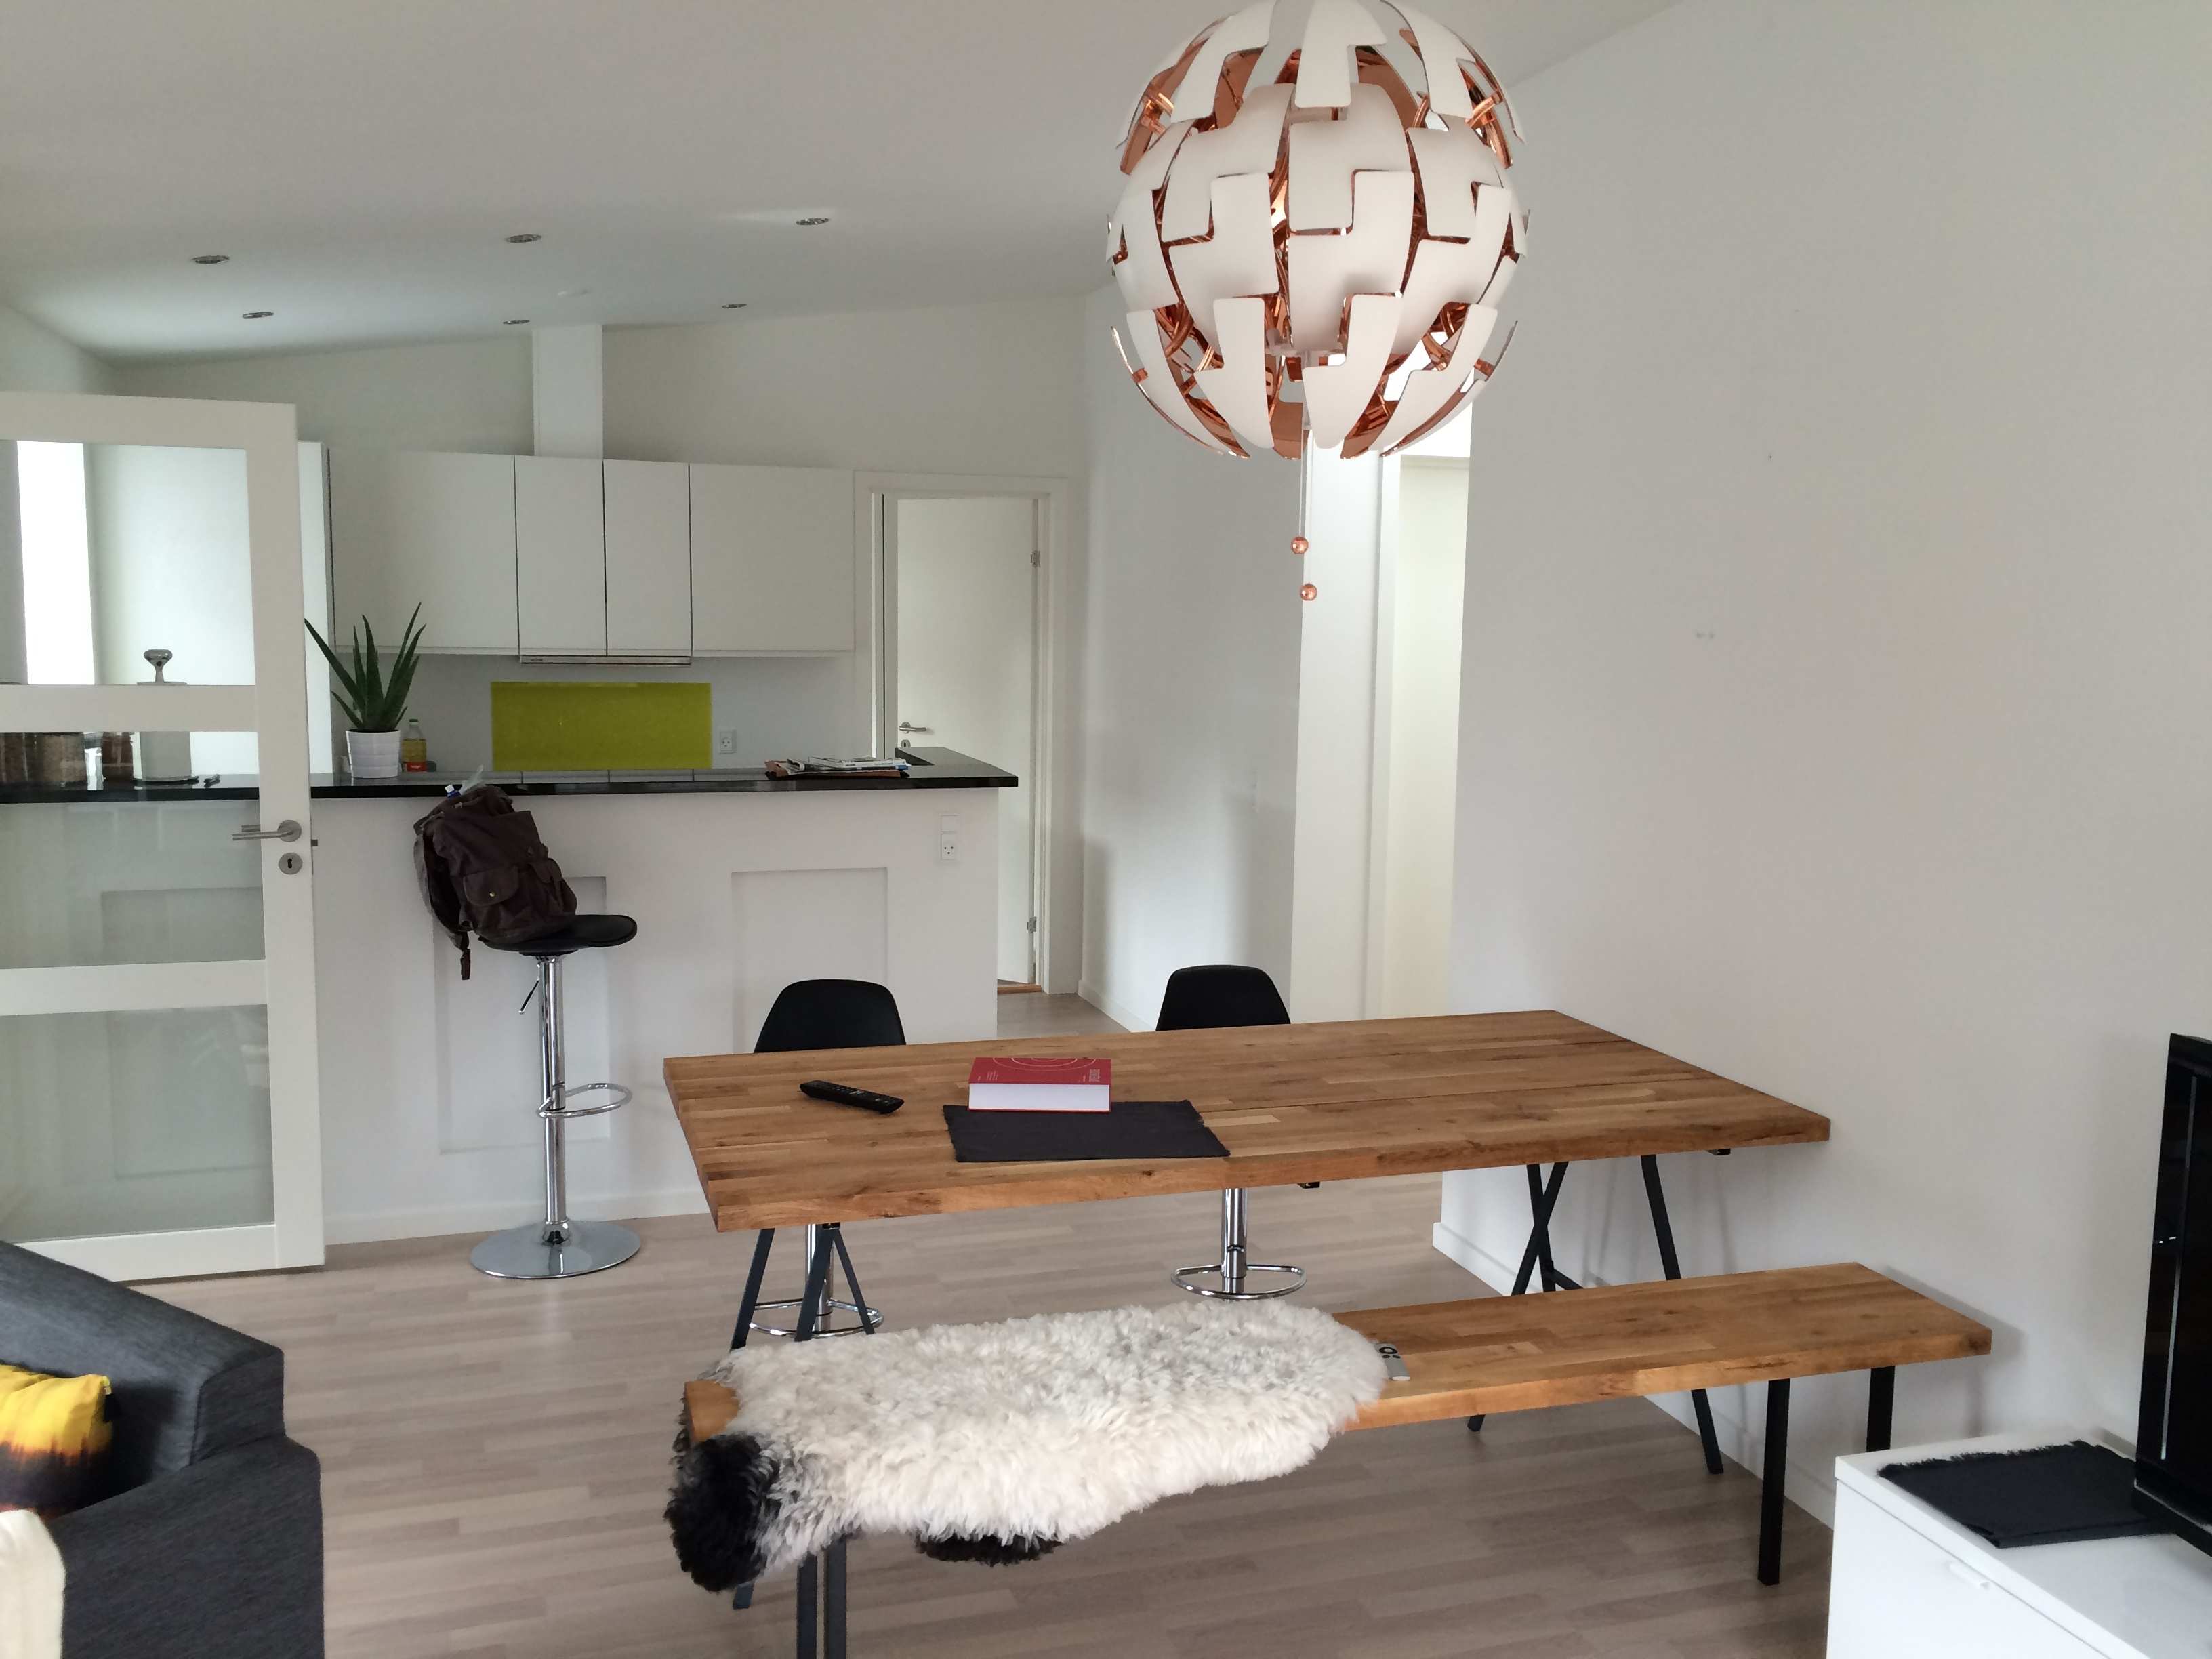
\includegraphics[width=.4\textwidth]{figures/roomOriginal.jpg}}
\end{figure}
\begin{figure}
\centering
\subfigure[0 bytes data gemt]{\label{fig:Room1char}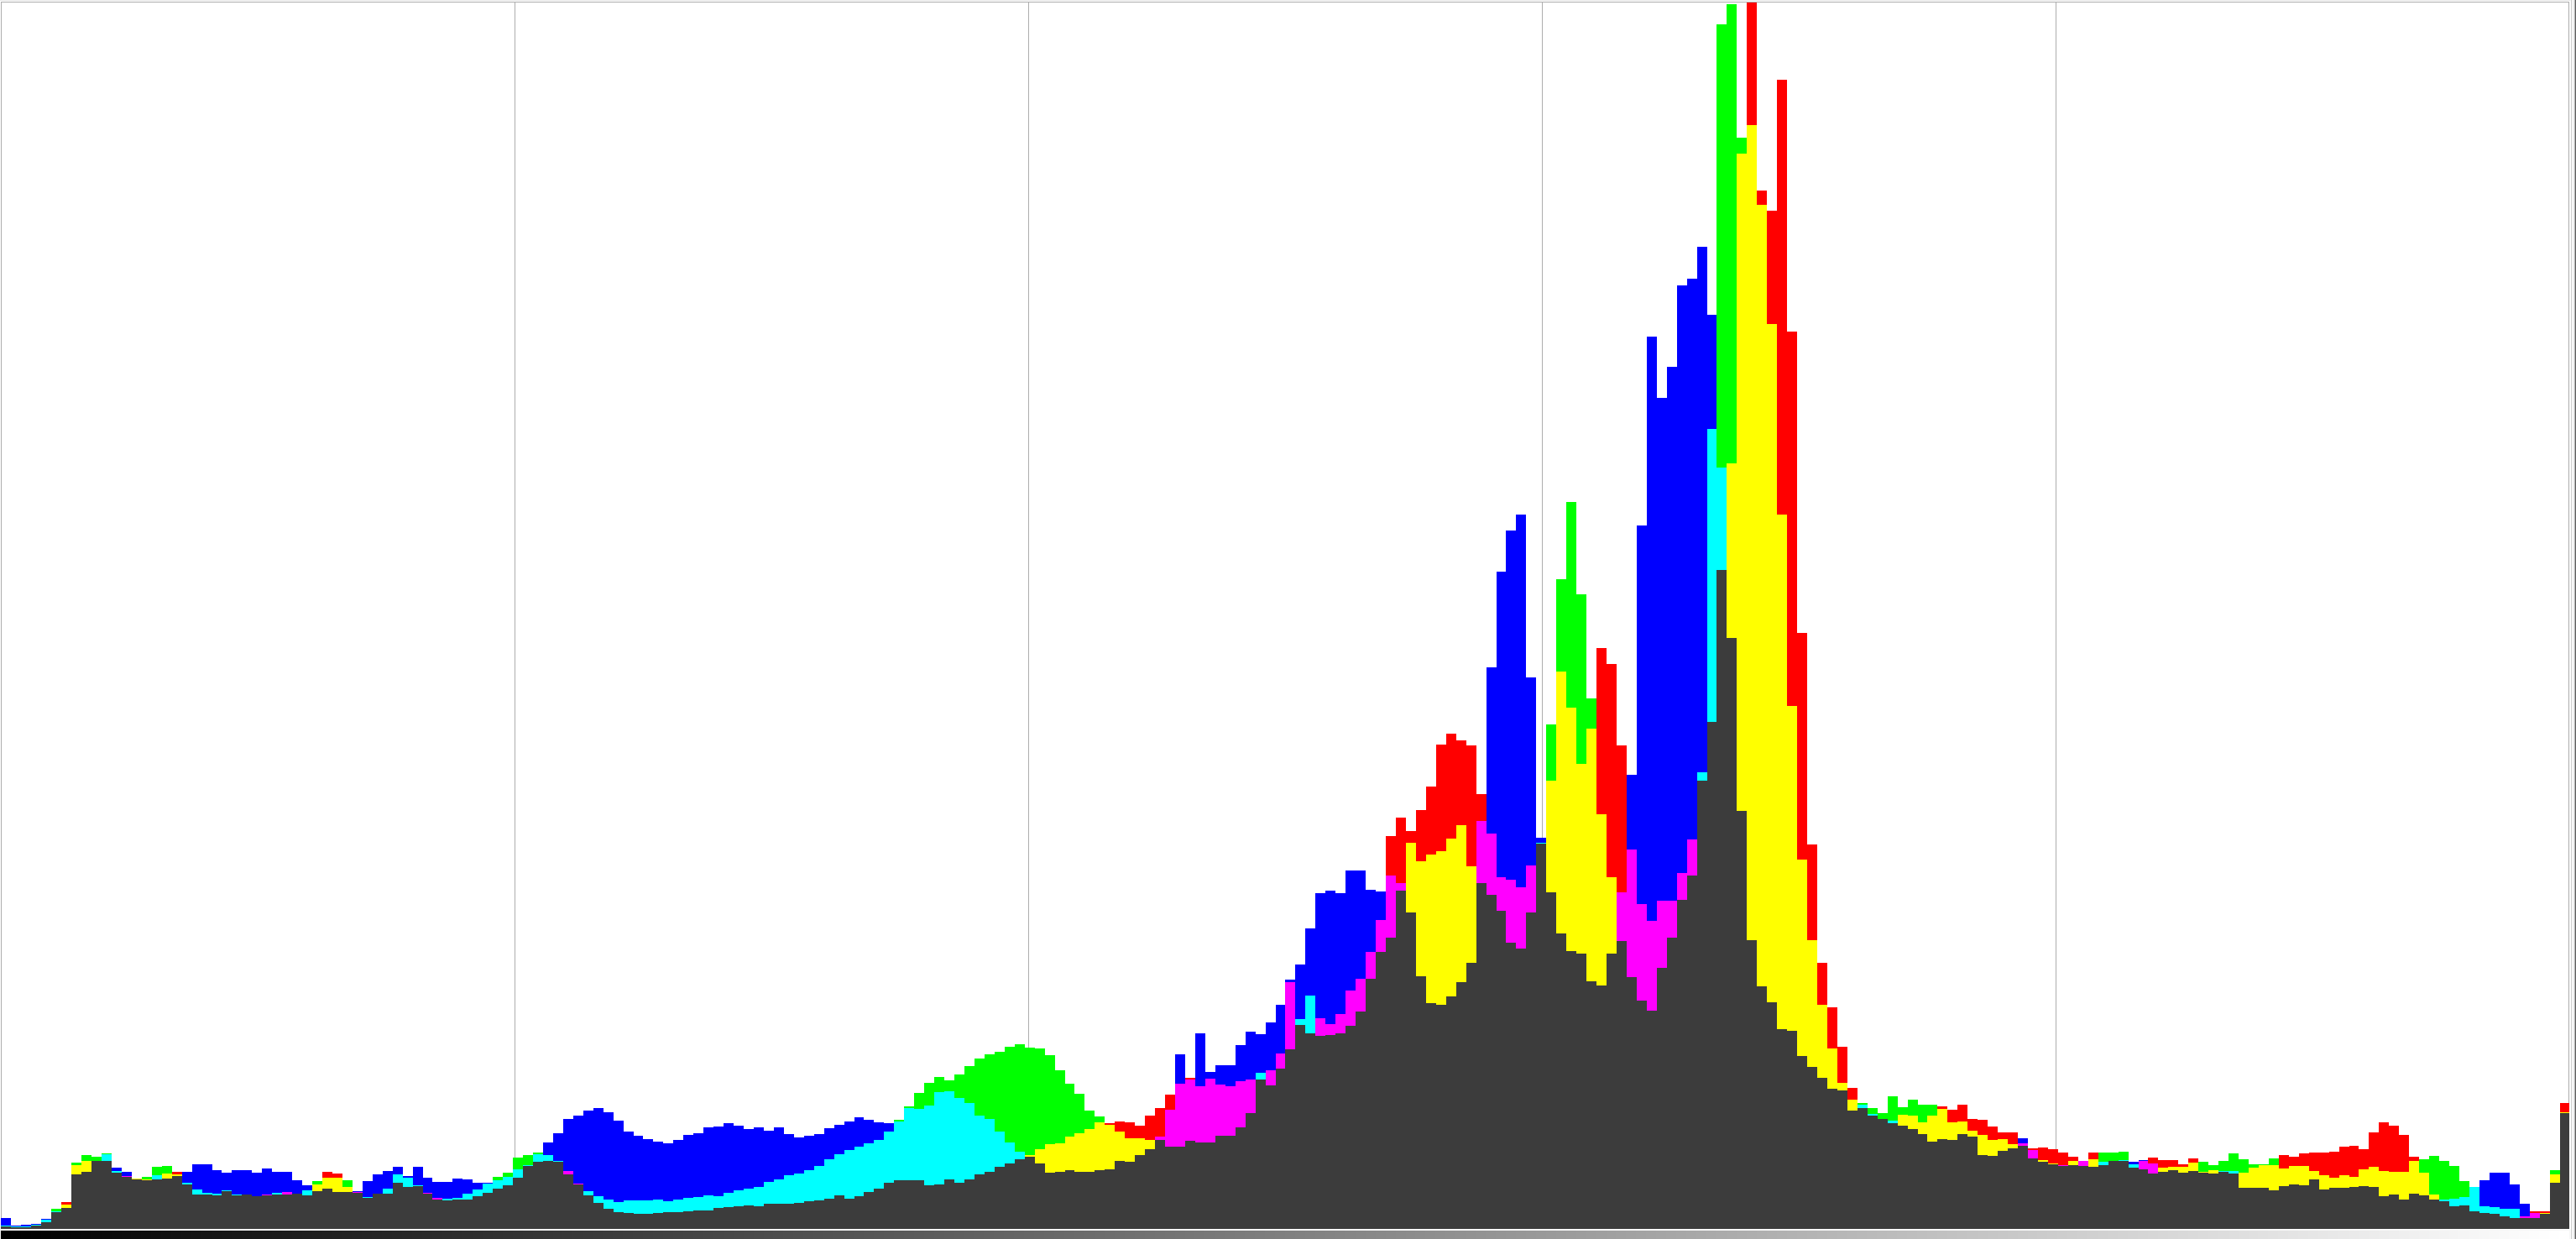
\includegraphics[width=.4\textwidth]{figures/room1char.png}}
\subfigure[2896 bytes data gemt]{\label{fig:RoomIntro}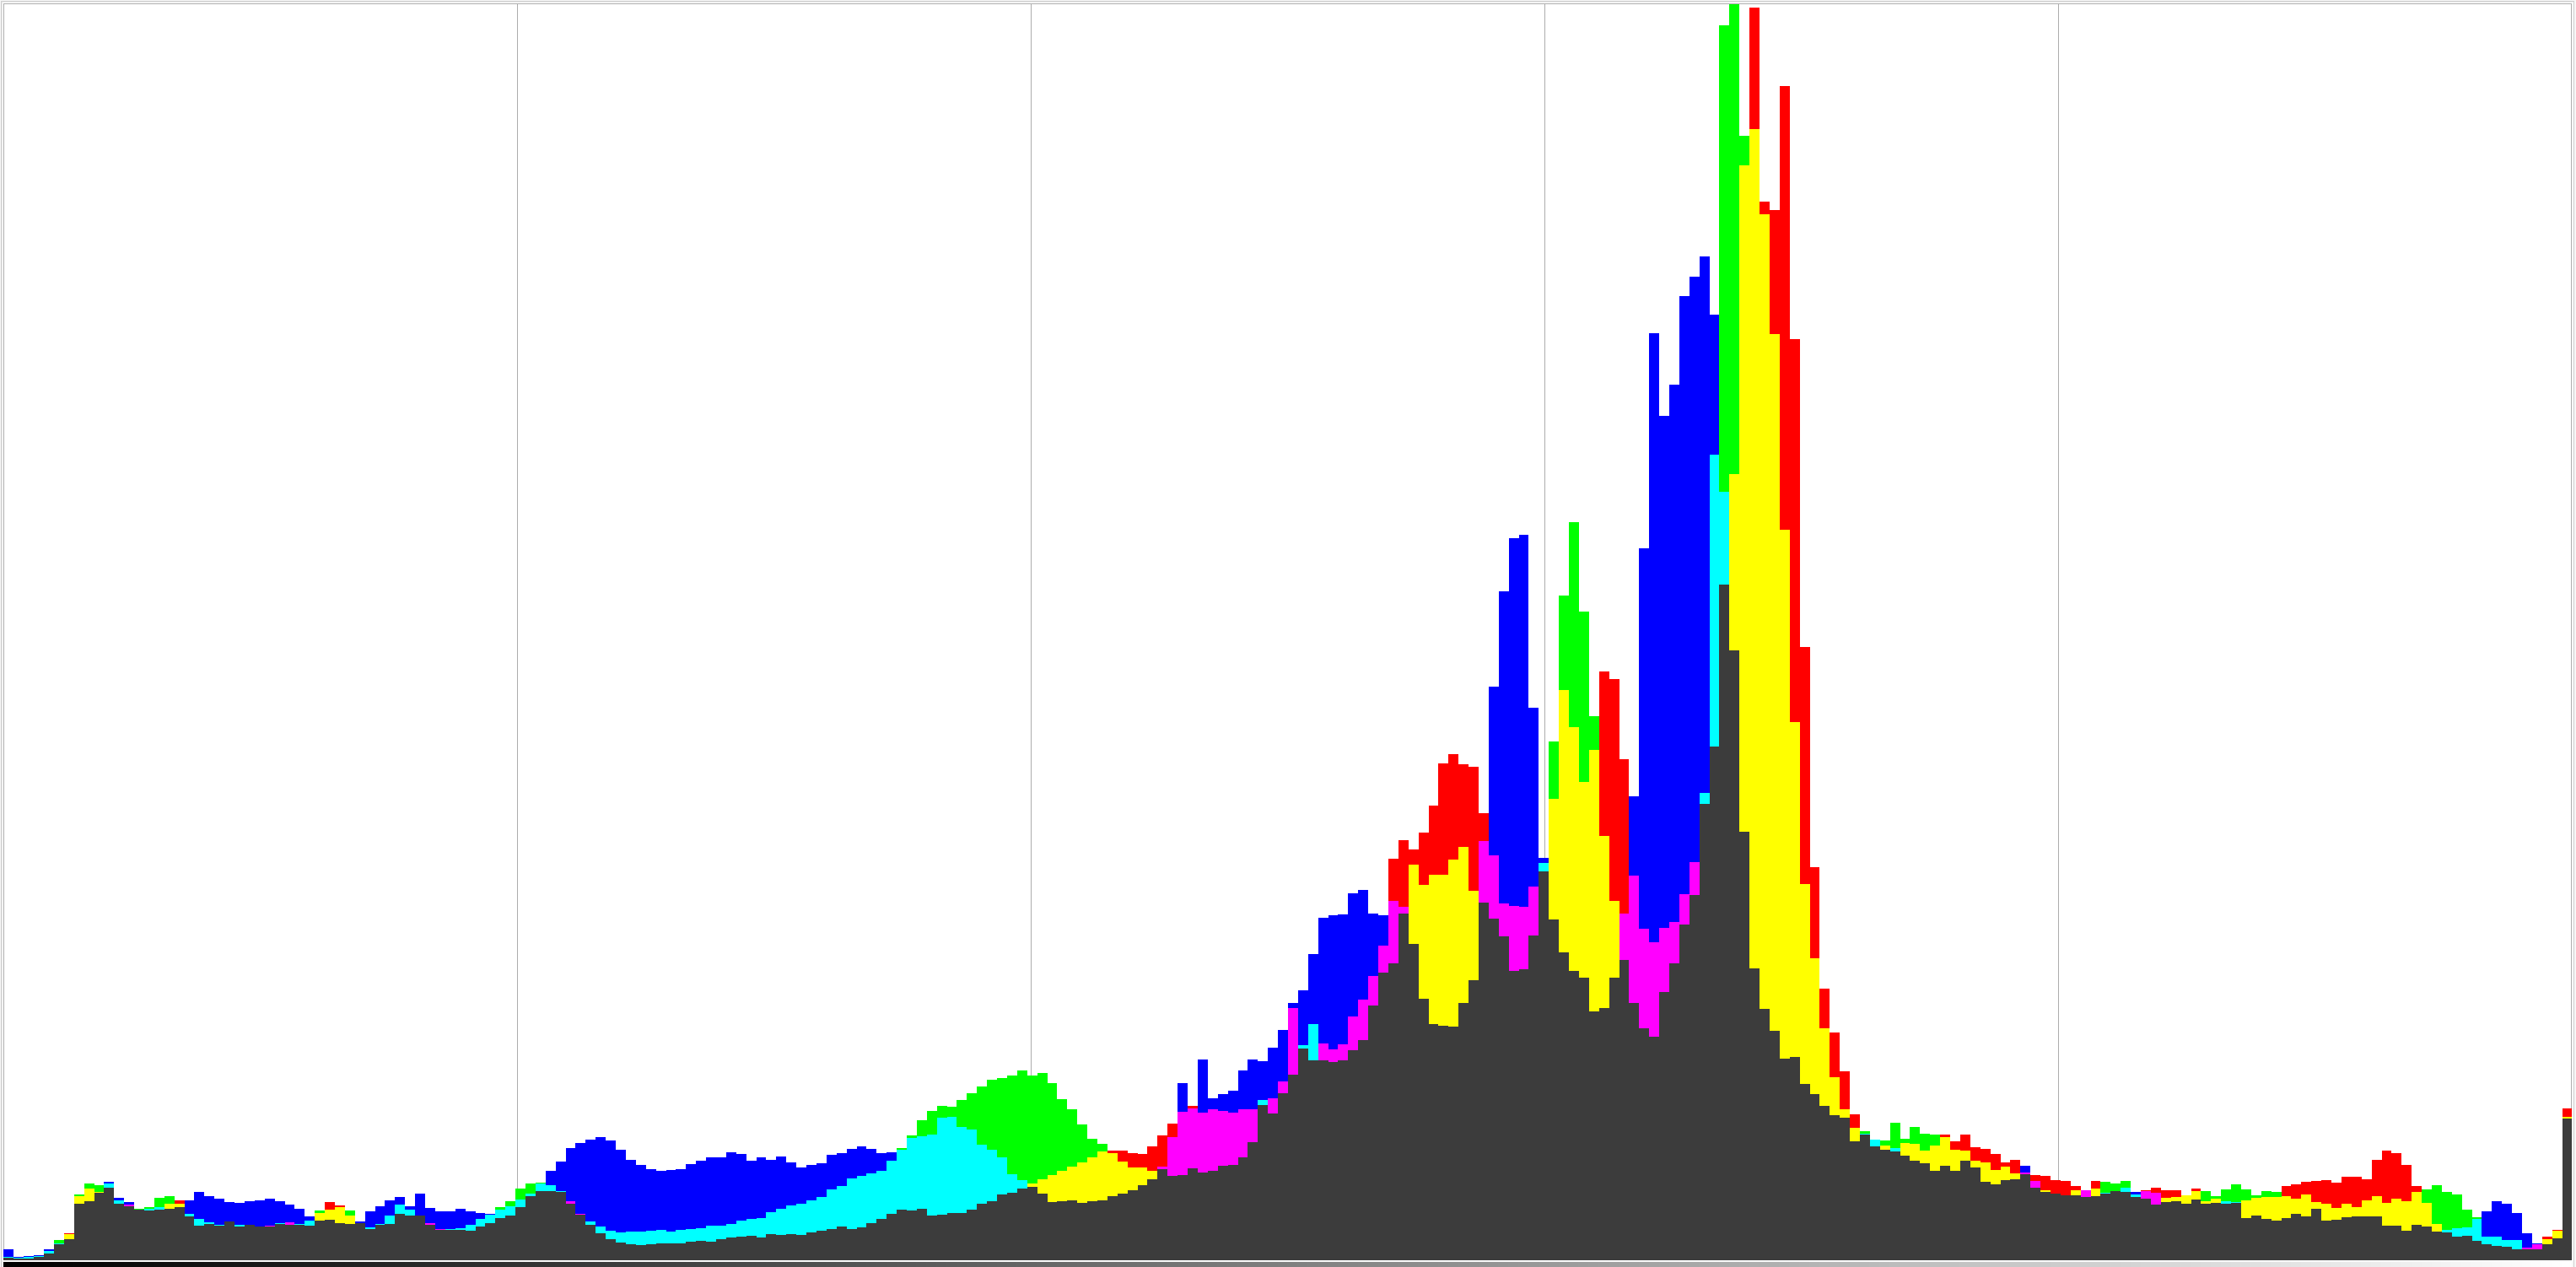
\includegraphics[width=.4\textwidth]{figures/roomEncodedIntroToSteg.png}}
\caption{Sammenligning af farvehistogram}
\end{figure}
\note{Stego intro is 2896 bytes or 2.896 kilobyte}
\end{frame}

\begin{frame}{Sammenligning med original billede}
\begin{figure}
\centering
\subfigure[Original]{\label{fig:a}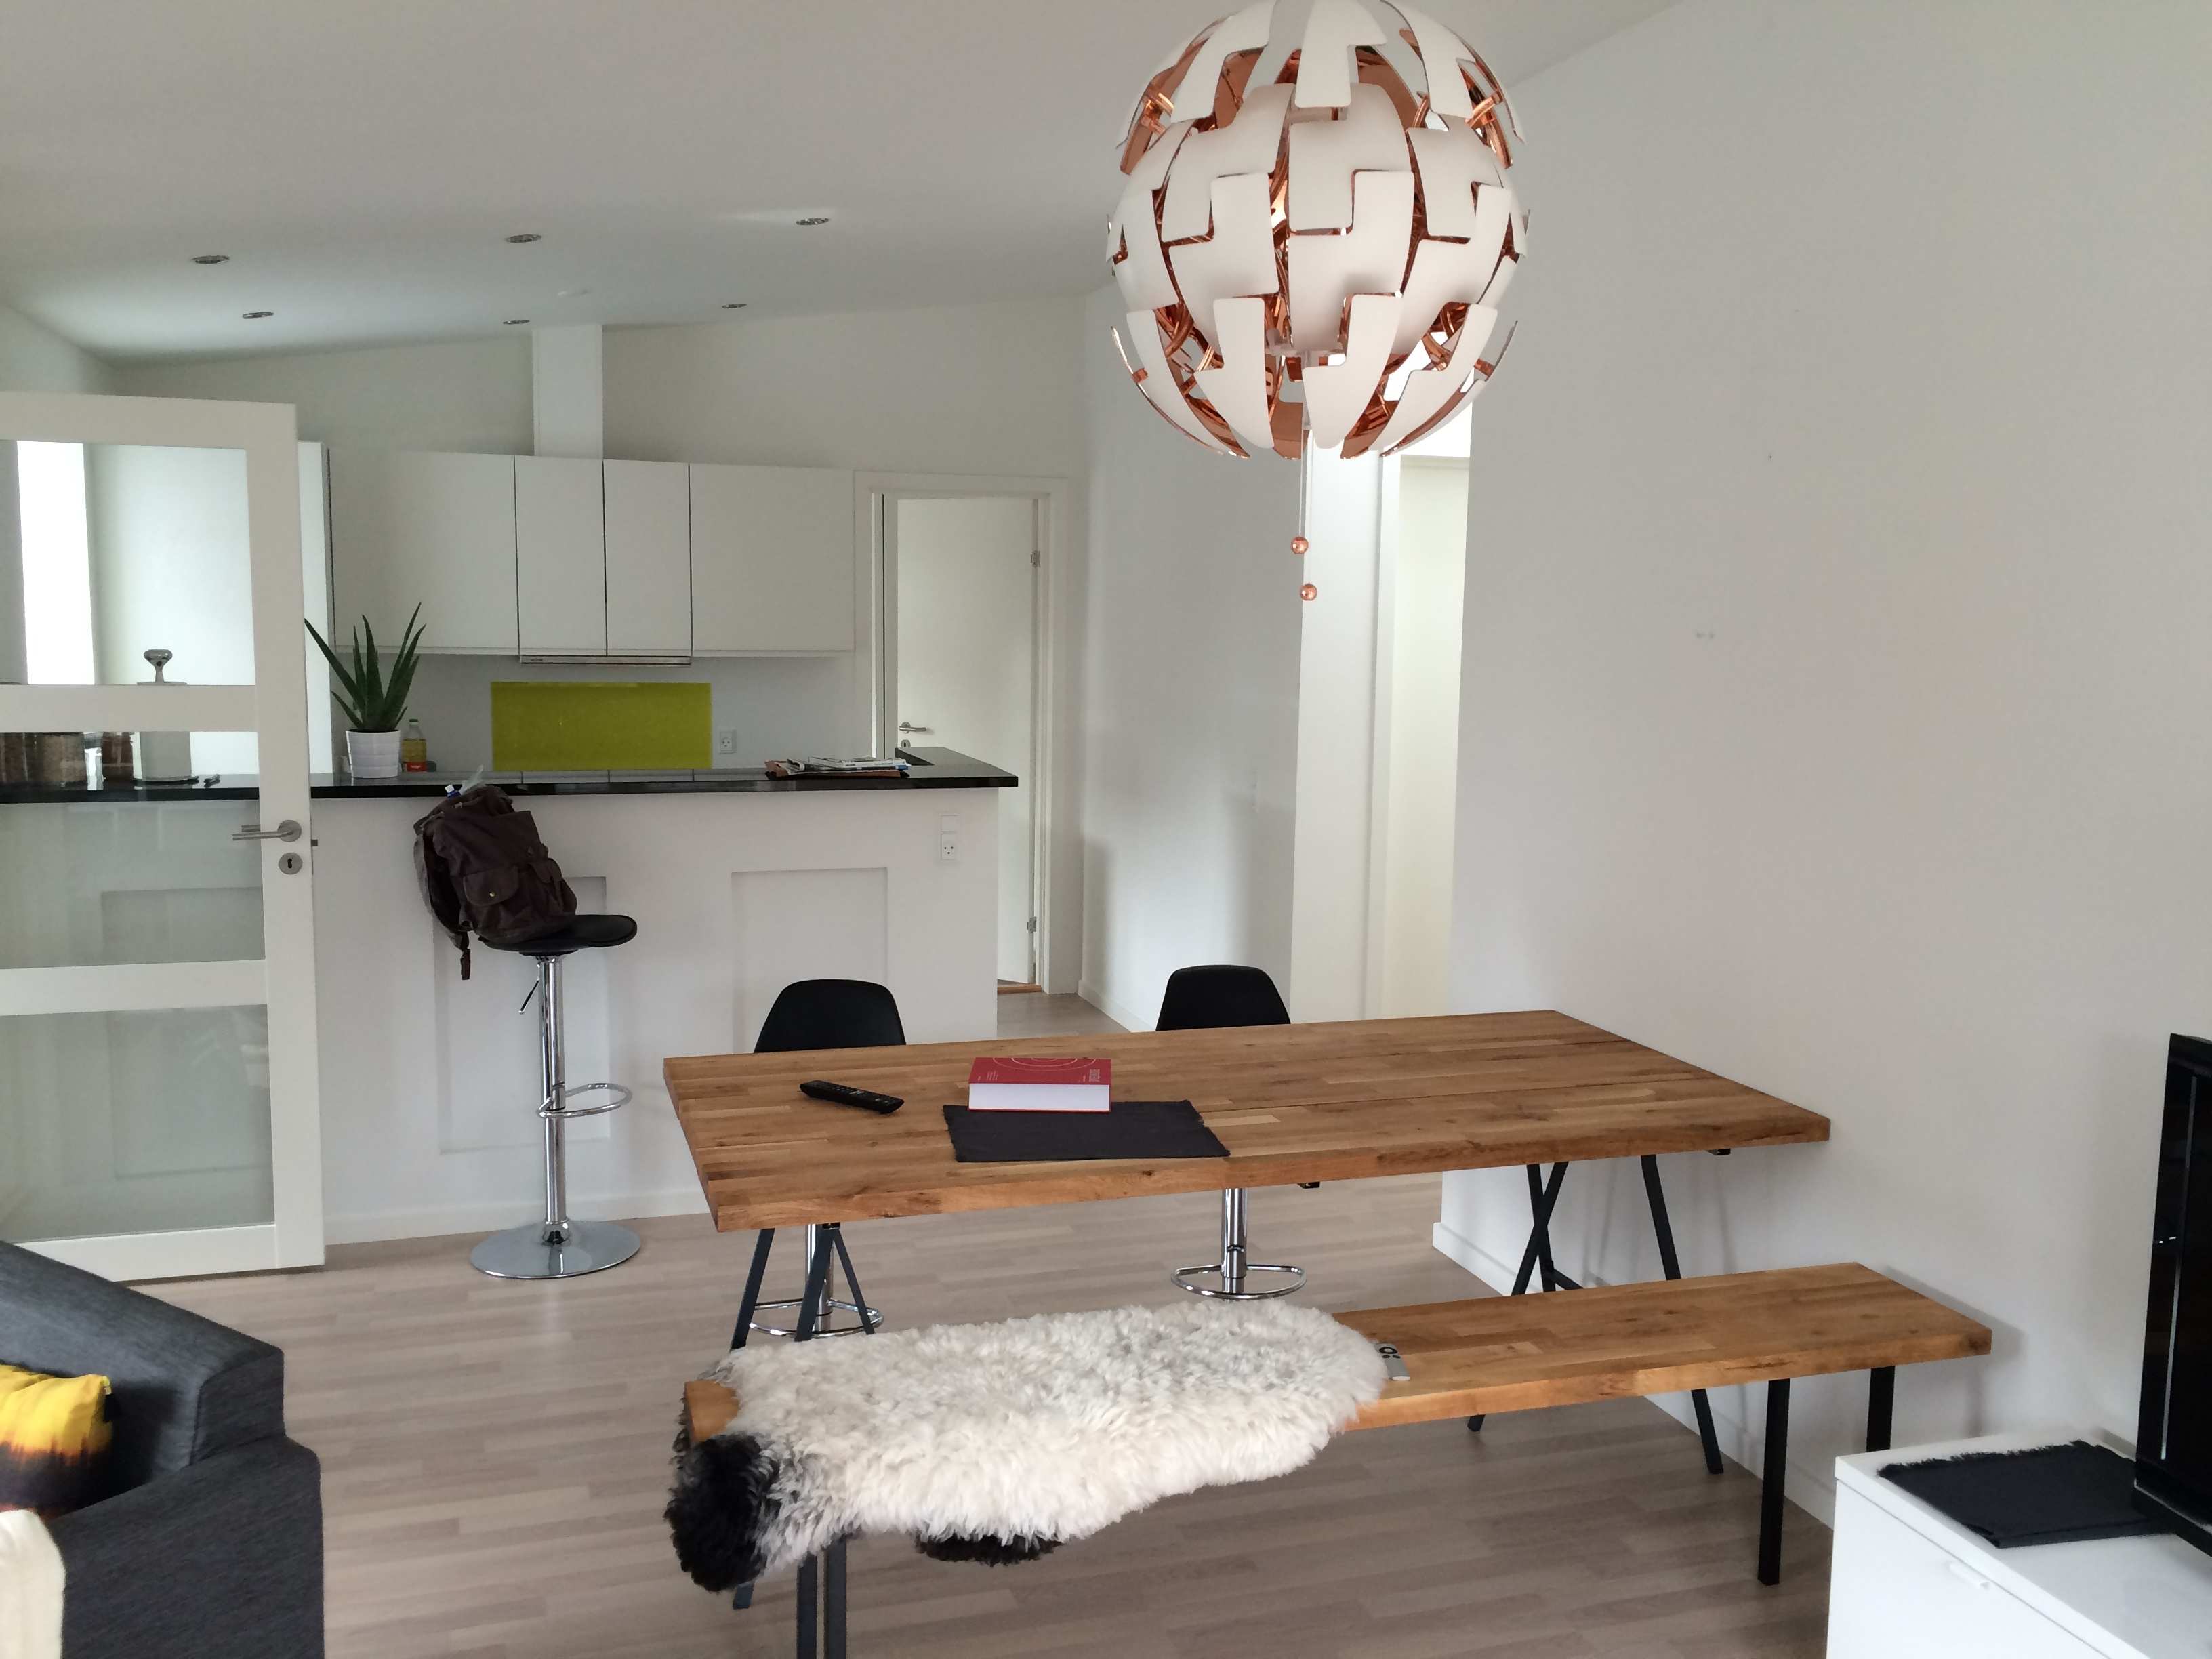
\includegraphics[width=.3\textwidth]{figures/roomOriginal.jpg}}
\end{figure}
\begin{figure}
\centering
\subfigure[2896 bytes vs. original]{\label{fig:b}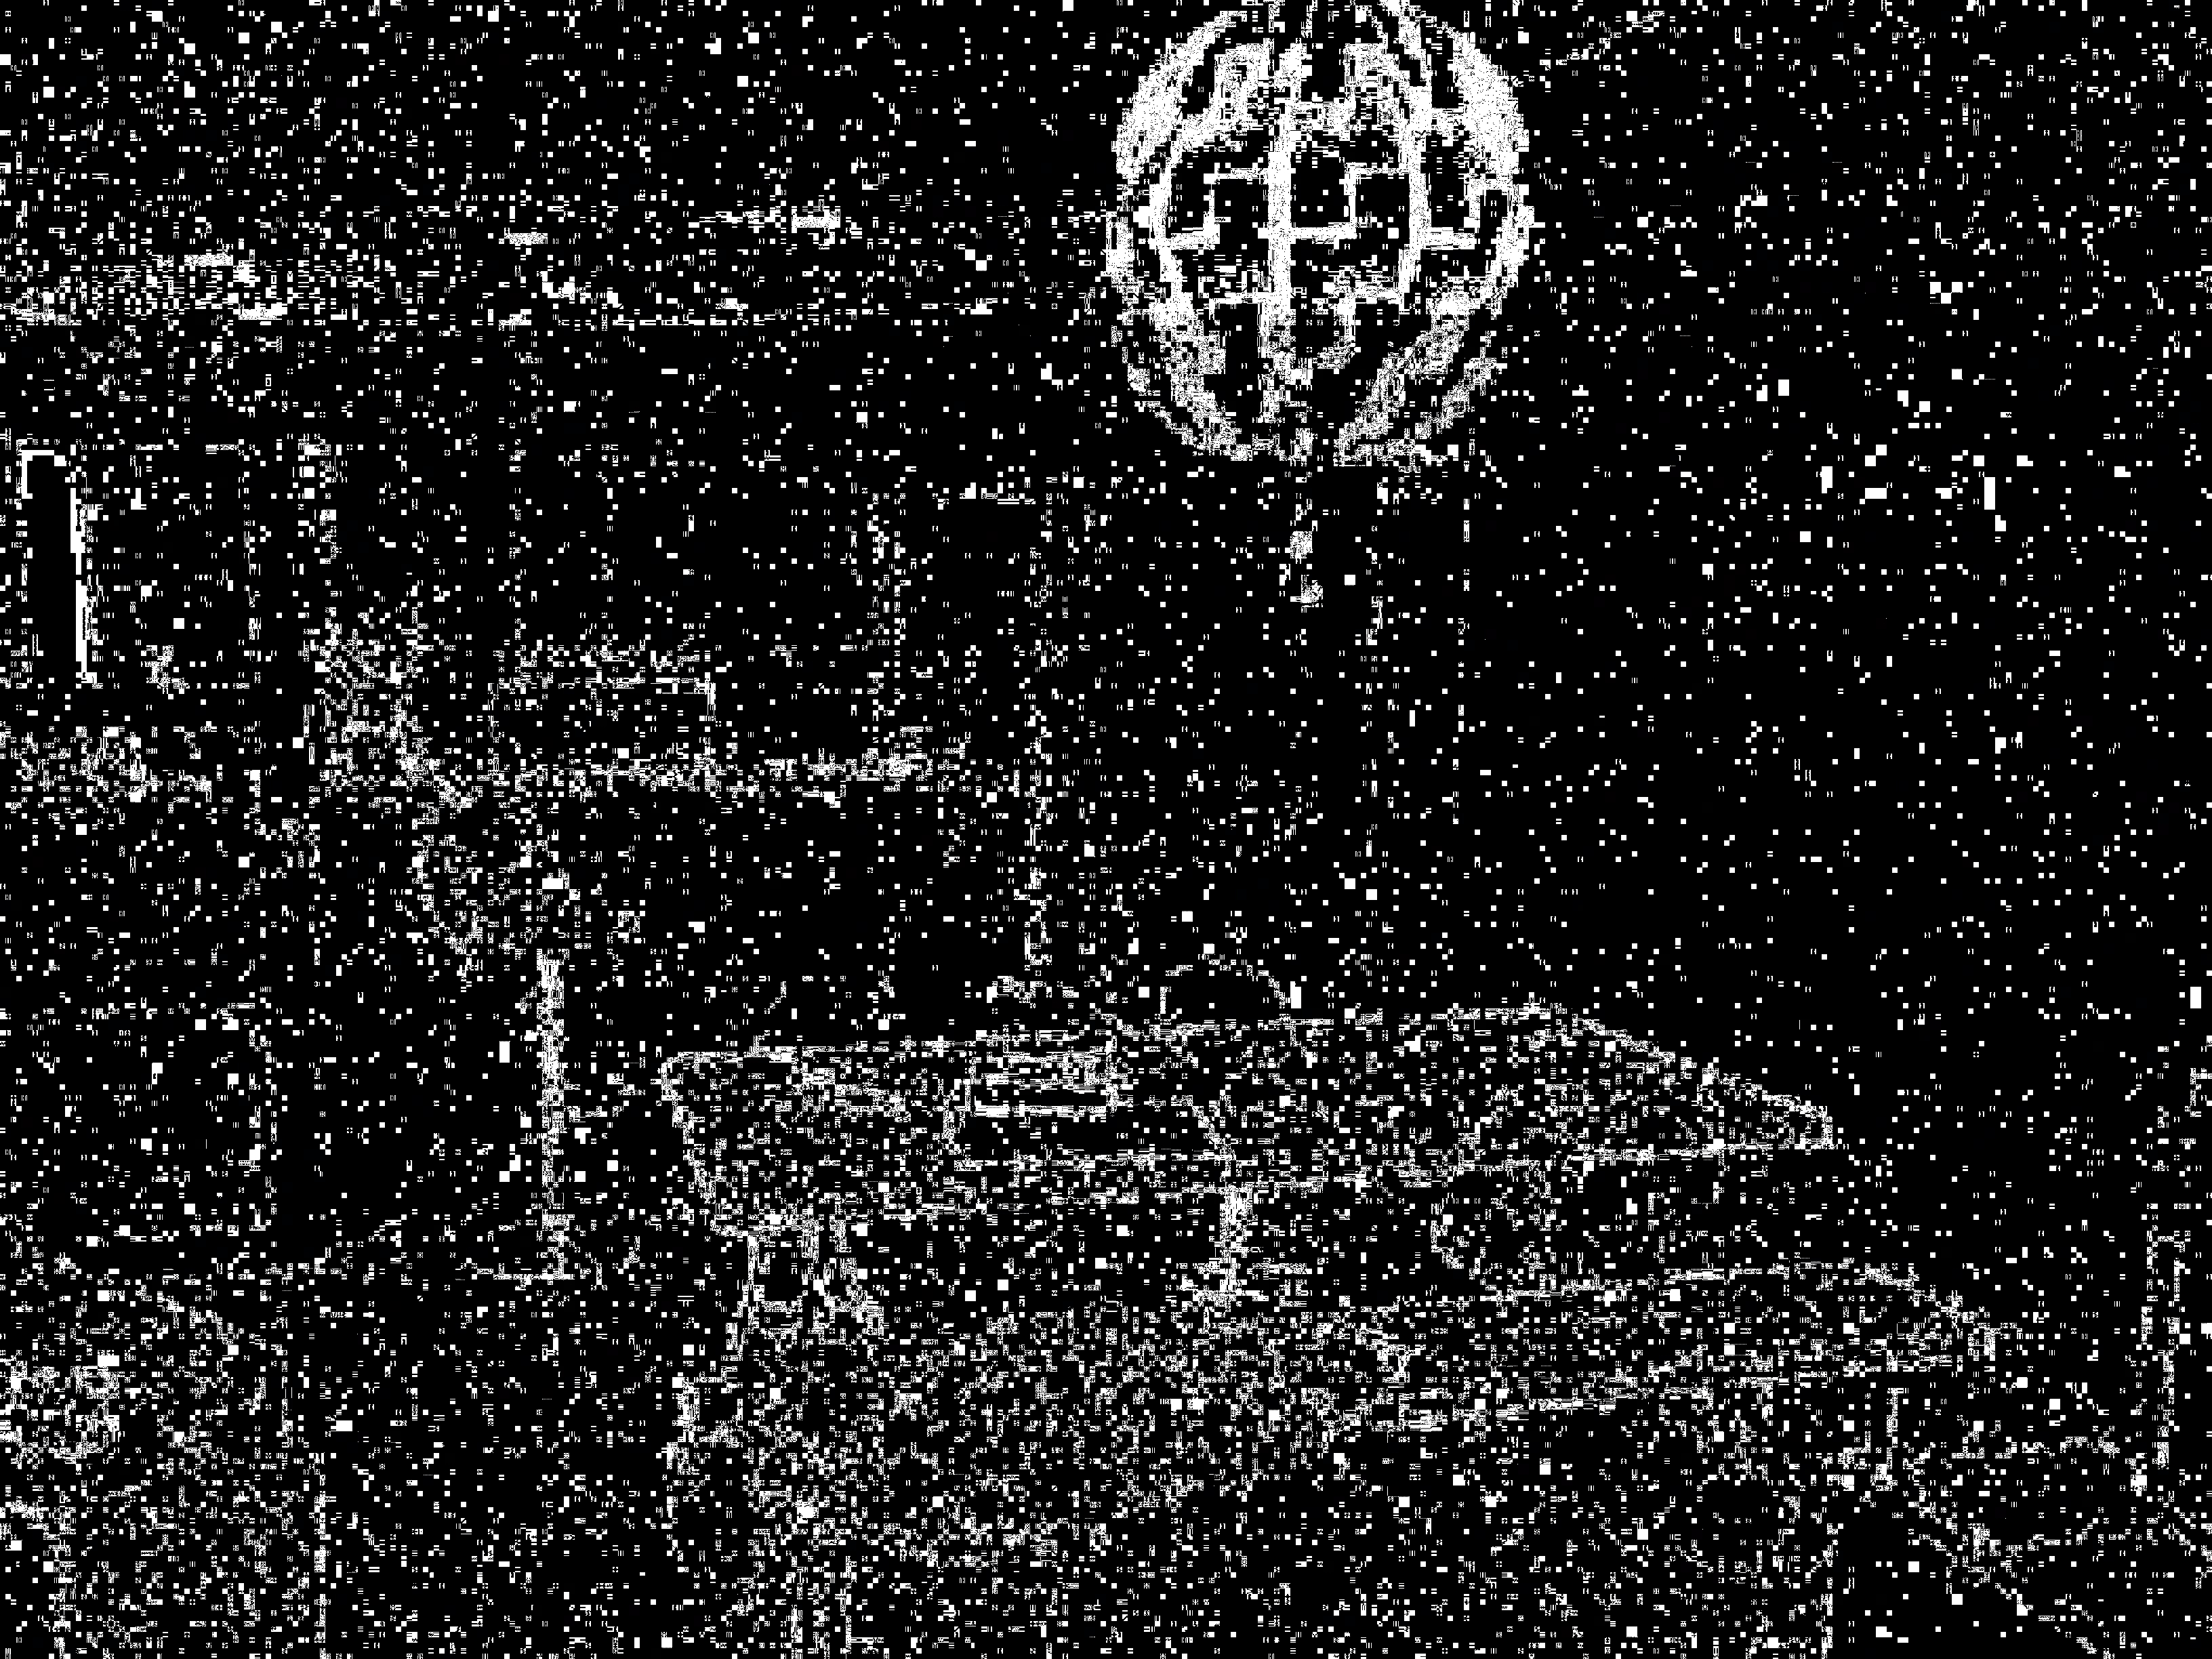
\includegraphics[width=.35\textwidth]{figures/introToStegovs1chardiff.jpg}}
\subfigure[500 bytes vs. original]{\label{fig:a}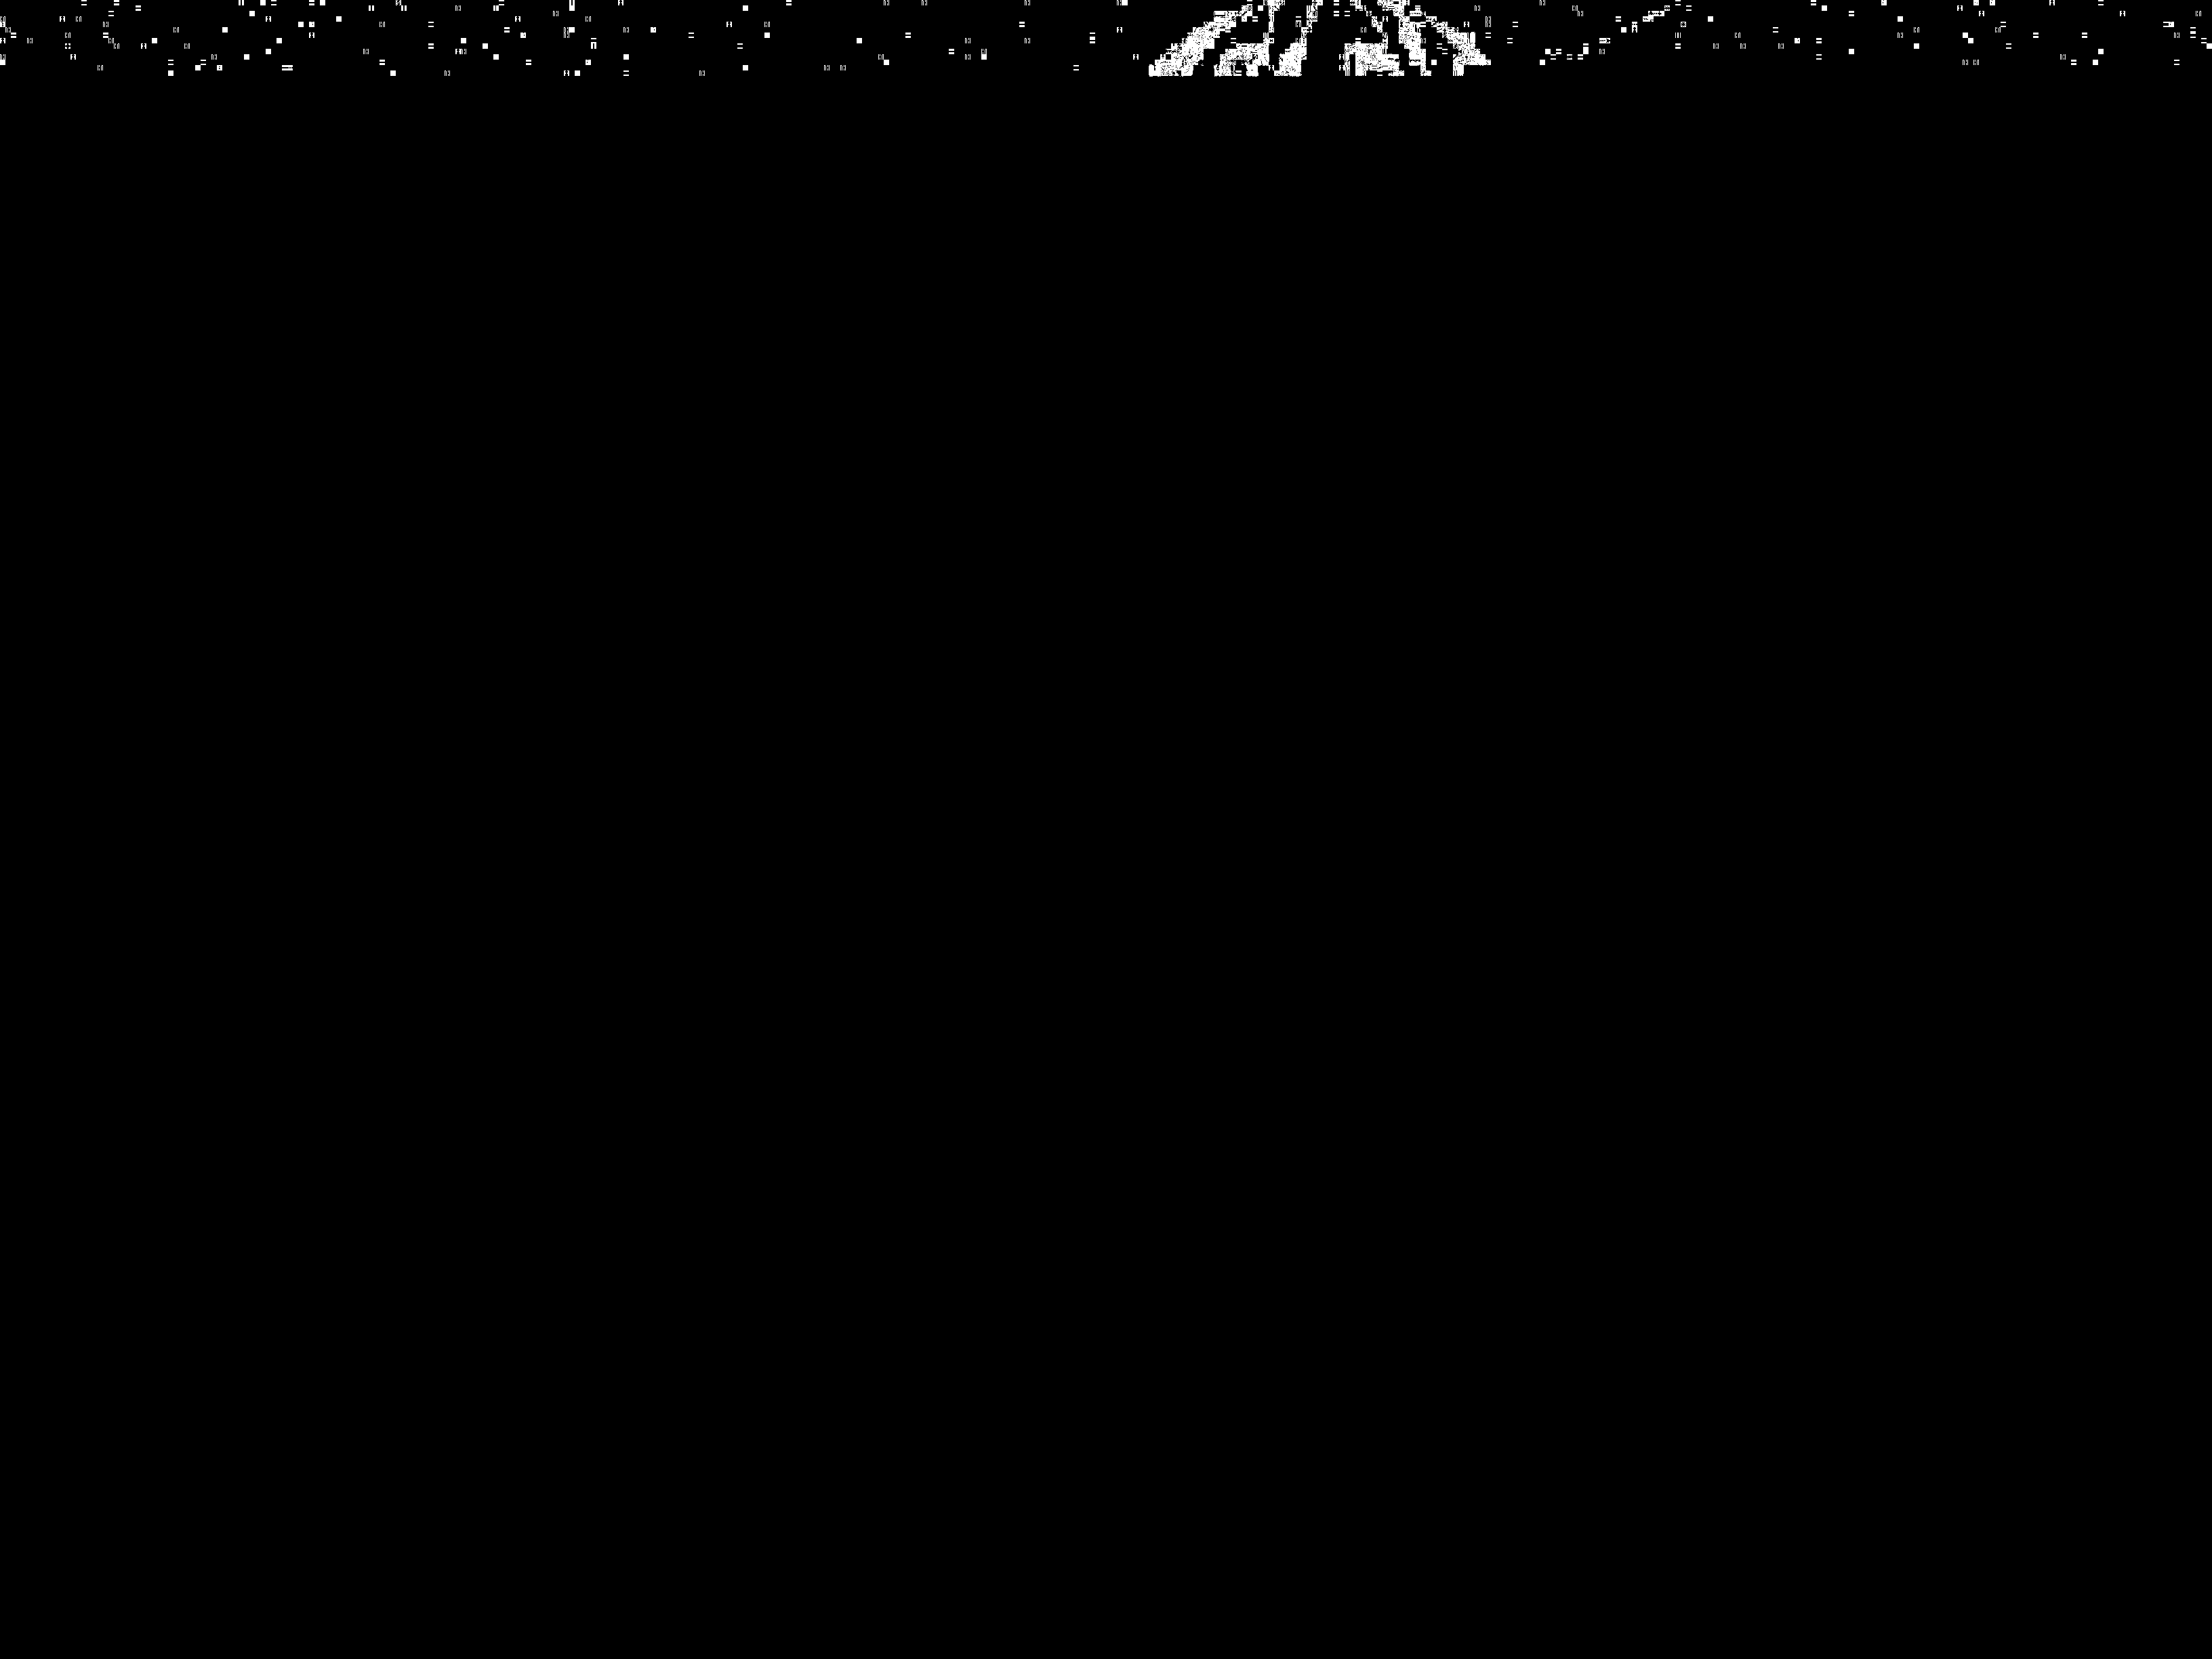
\includegraphics[width=.35\textwidth]{figures/loremIpsum1paragraphvs1chardiff.png}}
\caption{Sammenlligning af billeder}
\end{figure}
\note{
Lorem Ipsum 1. paragraph is 500 bytes 
Stego intro is 2896 bytes}
\end{frame}
	
\begin{frame}{LSB forstærkning}
	LSB forstærkning
	\begin{itemize}
		\item Fjern de 7 højtstående bits
		\item Alle bytes har nu værdien 0 eller 1
		\item Alle bytes ganges med 255
	\end{itemize}
\end{frame}

\begin{frame}{LSB forstærkning}
\begin{figure}
\centering
\subfigure[Grid LSB encoded 20kb]{\label{gridLSBencode}
\includegraphics[width=.4\textwidth]{figures/20kbLSBencoded_LSB.png}}
\end{figure}
\end{frame}

\begin{frame}{LSB forstærkning}
\begin{figure}
\centering
\subfigure[Original]{\label{fig:Room}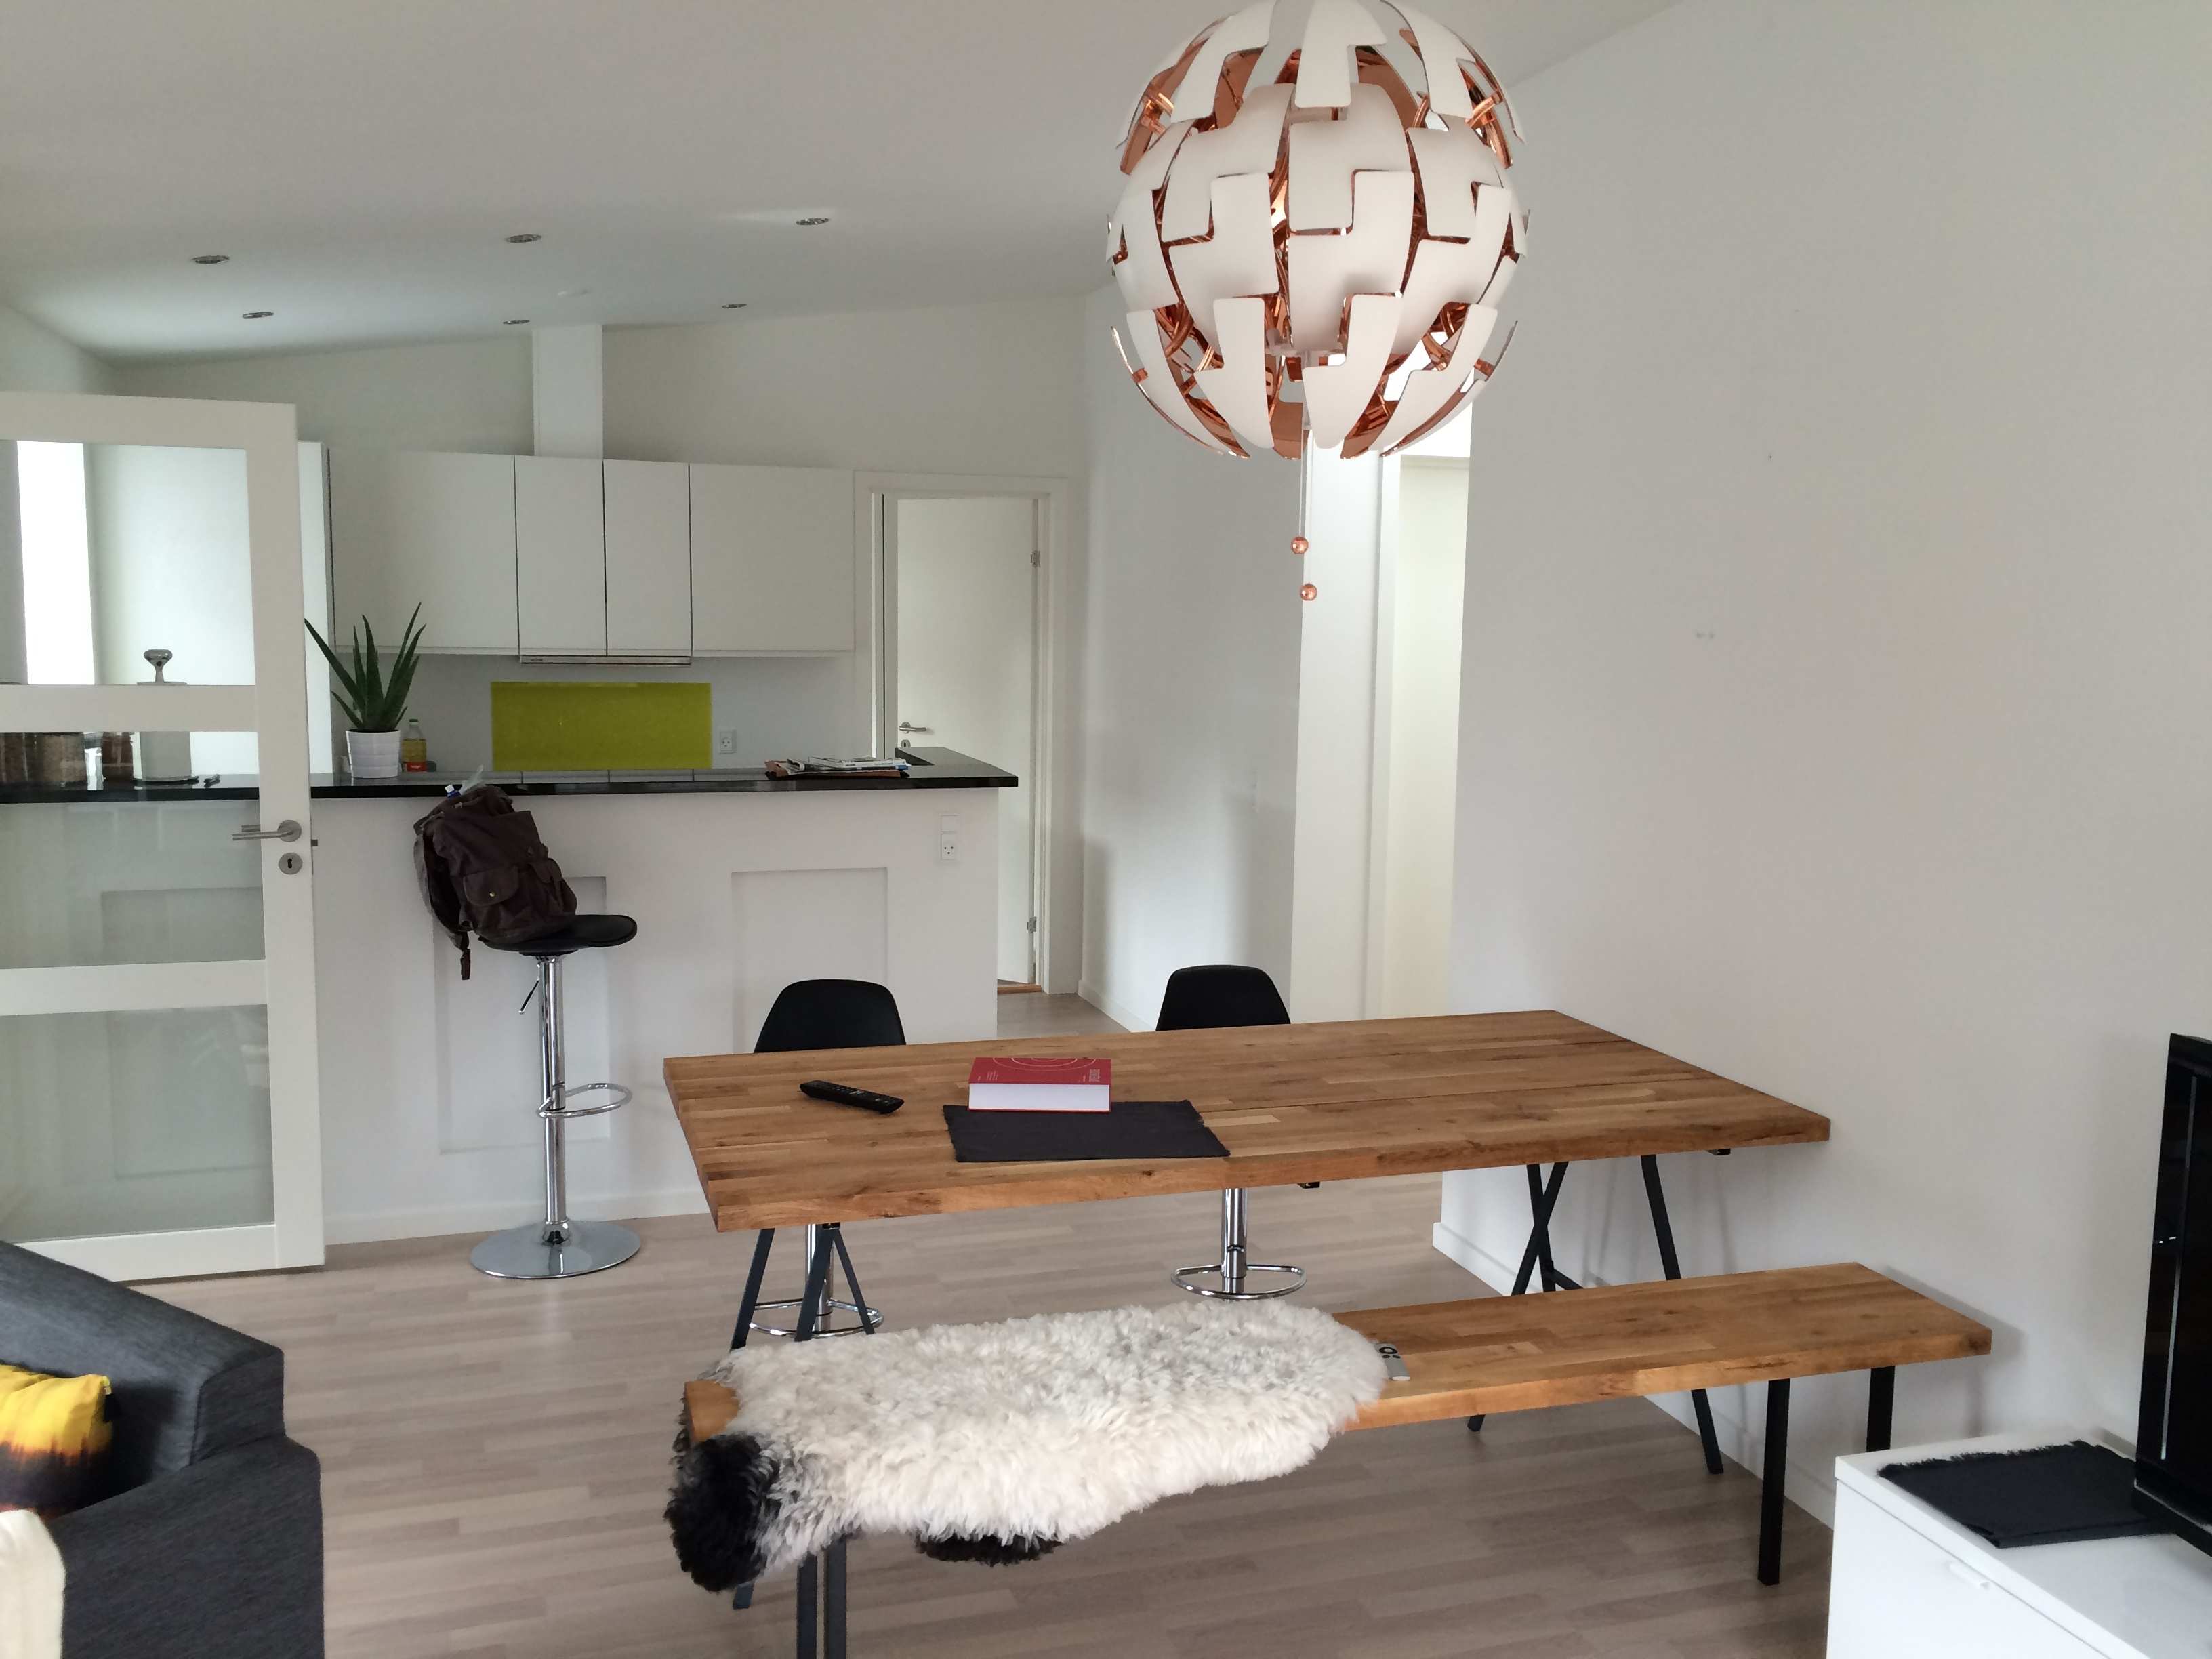
\includegraphics[width=.45\textwidth]{figures/roomOriginal.jpg}}
\subfigure[Original LSB enhanced]{\label{fig:Room}
\includegraphics[width=.45\textwidth]{figures/roomOriLSB.jpg}}
\end{figure}
\end{frame}

\begin{frame}{LSB forstærkning}
\begin{figure}
\centering
\subfigure[Original LSB forstærket]{\label{fig:Room}
\includegraphics[width=.45\textwidth]{figures/room1charLSBEnhanced.png}}
\subfigure[2896 bytes LSB forstærket]{\label{fig:Room}
\includegraphics[width=.45\textwidth]{figures/roomIntroLSB.jpg}}
\caption{Begge billeder}
\end{figure}
\note{Stego intro is 2896 bytes or 2.896 kilobyte
Looks ugly because of our JPEG encoder}
\end{frame}

\begin{frame}{Brute-decoding}
	Brute-decoding
		\begin{itemize}
		\item Decode billedet uden at vide længde eller modulo
		\item Prøv alle modulo-værdier
		\end{itemize}
\end{frame}

\begin{frame}{Brute-decoding}
TODO: Insert picture of brute-decoding tests
\end{frame}

\begin{frame}{Signatur}
	Signatur af vores program
		\begin{itemize}
		\item Første 16 bits af scan datas ikke-nul værdier
		\item Altid indkodet med modulo 4
		\end{itemize}
\end{frame}

\begin{frame}
TODO: Insert pictures of decoding of first 16bits
\end{frame}o